%% CloudKC-Bench — full paper (maam-spec structure), IEEEtran conference.
%% Compiles on Overleaf as-is. Figures in ./figures/ (vector PDFs).
\documentclass[journal]{IEEEtran}
\usepackage{cite}
\usepackage{amsmath,amssymb}
\usepackage{graphicx}
\usepackage{booktabs}
\usepackage{array}
\usepackage{url}
\usepackage[hidelinks]{hyperref}
\graphicspath{{figures/}}
\newcommand{\cmark}{\ensuremath{\checkmark}}
\newcommand{\xmark}{\ensuremath{\times}}

\begin{document}

\title{CloudKC-Bench: An Open Benchmark for LLM Cross-Domain\\Correlation in AWS Kill-Chain Reconstruction}

\author{\IEEEauthorblockN{Atishay Jain, Anna M., and S.~Nagasundari}
\IEEEauthorblockA{Centre for Information Security, Forensics and Cyber Resilience (ISFCR)\\
PES University, Bengaluru, India\\
atishay.offical@gmail.com}}

\maketitle

\begin{abstract}
Attacks on cloud infrastructure rarely appear as a single anomalous event; a modern multi-stage
kill chain scatters its evidence across heterogeneous logs---administrative API activity, network
flows, storage operations, and compute events---that share no common key. Whether large language
models (LLMs) can correlate across these logs to rebuild the attack, and whether they do so better
than simpler methods, is an open and largely unmeasured question. We present CloudKC-Bench, the
first open benchmark for AWS control-plane multi-stage kill-chain reconstruction: taxonomy-structured,
real-incident-grounded scenarios, each released with a machine-checkable ground-truth manifest and a
published, deterministic matching function. Using the benchmark we run a pre-registered four-arm
ablation (multi-agent LLM, single-agent LLM, single agent without a pre-filter, and a rules-only
correlator) plus an independent community Sigma baseline, holding model, telemetry, and compute
fixed. On a real-AWS run with Qwen2.5-32B, the LLM detects cross-domain attack \emph{events} at
higher precision than the rules (up to $1.00$ vs $0.65$ on multi-stage kill chains) but is markedly
worse at exact ATT\&CK-\emph{technique} attribution (recall $\sim$0.12 vs $0.87$); multi-agent
decomposition adds no measurable value over a single agent. All artifacts are released for
independent replication.
\end{abstract}

\begin{IEEEkeywords}
Cloud security, large language models, security benchmark, MITRE ATT\&CK, kill-chain reconstruction,
threat detection, Amazon Web Services, multi-agent systems, reproducibility, security evaluation.
\end{IEEEkeywords}

% ====================================================================
\section{Introduction}
Cloud computing is now the standard way organizations run their software, and its importance keeps
growing. Gartner expects worldwide spending on public cloud services to reach US\$723.4 billion in
2025, up 21.5\% from US\$595.7 billion in 2024, driven in large part by the rise of
artificial-intelligence workloads~\cite{gartner25}. As companies move not just their data and
computing but also their identities, controls, and administrative tools into the cloud, the
\emph{control plane}---the set of interfaces used to create, configure, and manage cloud
resources---becomes the main place where both business value and security risk now sit.

This shift has a well-known cost. Gartner predicts that through 2025, about 99\% of cloud security
failures will be the customer's own fault, usually caused by misconfiguration or poorly managed
access rather than by the cloud provider~\cite{gartner99}. Real incidents confirm this. In the 2019
Capital One breach, an attacker combined a web vulnerability with stolen machine credentials to copy
out large amounts of data~\cite{capitalone}. Campaigns such as SCARLETEEL~\cite{scarleteel} and
TeamTNT~\cite{teamtnt} moved step by step through reconnaissance, credential theft, privilege
escalation, and resource abuse inside cloud accounts. In every case the attack was not a single
strange event but a chain of steps, and the evidence for those steps was spread across several
different logs.

Because of this, researchers have begun to ask whether large language models (LLMs) can help security
teams. Recent surveys describe a fast-growing body of work that uses these models for reading logs,
spotting anomalies, checking for vulnerabilities, and assisting analysts~\cite{llmsurvey1,
llmsurvey2, llmsurvey3}. The idea is appealing: a language model can read messy, mixed data and
reason about it in plain language, possibly replacing the rigid, hand-written rules that most
security tools rely on today. Some cloud-focused systems have already tried this, for example by
writing detection rules from threat reports~\cite{llmcloudhunter} or by adding a language model to
explain the alerts of a traditional detector~\cite{huntgpt}.

Rebuilding a multi-step cloud attack, however, is much harder than labeling a single event, and it is
exactly where the value of language-model correlation is least understood. The kill-chain idea,
introduced by Hutchins \emph{et al.}~\cite{hutchins} and made practical for the cloud by the MITRE
ATT\&CK framework~\cite{mitre}, describes an attack as an ordered set of stages: getting in, gaining
privileges, evading defenses, stealing credentials, exploring, moving sideways, stealing data, and
causing damage. In the cloud, each stage usually shows up in a different log---administrative actions
in CloudTrail, network traffic in VPC Flow Logs, file operations in storage logs, and machine events
in compute logs. These logs share no common key and arrive at different, unpredictable times, so
putting the chain back together means connecting clues \emph{across} logs, not within a single
one~\cite{wilkens, hetfusion}.

Despite the excitement, claims about language models in this area are often made without the
safeguards that would let others check them. Results are frequently reported without fair baselines
that separate the model's contribution from the rest of the system, without shared and clearly
labeled datasets, and without admitting that the model's answers can change from run to run---the
kind of pitfalls shown to inflate results across security machine learning~\cite{arp22}. On top
of this, no public benchmark exists for rebuilding AWS control-plane kill chains with answers a
computer can check automatically. Existing benchmarks target a different platform, a different
task---such as malware analysis, threat-intelligence question answering, architecture modeling, or
insider threat---or they measure how well a system \emph{writes} detection rules rather than how well
it \emph{rebuilds} an attack~\cite{cybersoceval, excytin, orgforge, acseeval}. The community is
therefore missing both the \emph{tool} to measure whether language-model correlation really helps and
the \emph{method} to say which part of a system deserves the credit.

This paper closes that gap. We present CloudKC-Bench, an open, answer-checked benchmark for rebuilding
AWS control-plane multi-stage kill chains, and use it to run a carefully pre-planned, controlled
comparison of four system variants---plus an independent rule-based baseline---on real AWS data,
reporting the results honestly whether or not the language model wins. The principal contributions of
this work are as follows.

\begin{itemize}
\item \textbf{C1.} \emph{CloudKC-Bench}, the first open benchmark targeting AWS control-plane
multi-stage kill chains, releasing taxonomy-structured, real-incident-grounded scenarios with
machine-checkable ground-truth manifests and a published, deterministic matching function.
\item \textbf{C2.} A pre-registered, controlled four-arm ablation on identical telemetry that
attributes any detection advantage to a specific layer---pre-filtering, the LLM, or multi-agent
decomposition---together with an independent community-Sigma baseline.
\item \textbf{C3.} A first-class cost-and-latency analysis of deterministic pre-filtering,
quantifying the trade-off between token expenditure and detection recall.
\item \textbf{C4.} A failure-mode taxonomy including technique-attribution confusion and a
model-scale analysis contrasting 7-billion- and 32-billion-parameter models on identical real-AWS
telemetry.
\item \textbf{C5.} A reproducibility artifact comprising the scenario generator, manifests, schema,
matching function, and analysis scripts, released to enable independent replication.
\end{itemize}

The remainder of this paper is organized as follows. Section~\ref{sec:bg} surveys the background.
Section~\ref{sec:framework} presents the CloudKC-Bench framework. Section~\ref{sec:impl} describes the
implementation. Section~\ref{sec:results} reports the experimental results. Section~\ref{sec:disc}
interprets the findings and their limitations, and Section~\ref{sec:conc} concludes.

% ====================================================================
\section{Background}\label{sec:bg}

\subsection{Fundamental Concepts}
Three ideas recur throughout this paper: the data a cloud platform produces, the way attacks are
described as staged sequences, and the recent use of language models to interpret security data. A
cloud account constantly produces \emph{telemetry}---records of what happened to its resources. On
Amazon Web Services, four sources carry most of the security signal: CloudTrail records
administrative API calls, VPC Flow Logs record network connections, storage access logs record object
operations, and compute logs record when machines are launched or terminated. Each source captures
only one slice of behavior, and no single source contains a whole attack. Attacks themselves are
usually described using the \emph{kill chain}~\cite{hutchins}, and the MITRE ATT\&CK
framework~\cite{mitre} turns this idea into a catalog of concrete \emph{techniques}, each mapped to a
tactical goal. Finally, large language models have recently been applied to security data, and broad
surveys report fast-growing work on log analysis, anomaly detection, and analyst
support~\cite{llmsurvey1, llmsurvey2, llmsurvey3}. Individually these concepts are mature; what
remains largely unstudied is their combination---using a model to rebuild an ATT\&CK-mapped kill
chain from several disconnected cloud logs at once---and whether doing so measurably helps.

\subsection{Existing Approaches}
Prior work on turning telemetry into detections falls into four families, and comparing them shows why
none yet solves the problem we target.

The first family is \emph{rule-based detection and event correlation}. In its simplest form it is
captured by the vendor-neutral Sigma standard~\cite{sigma}, whose strengths are transparency and low
cost but whose weakness is a high false-positive rate, because generic rules match the ordinary
administrative actions that attackers also use. To move beyond single events, security-information-and-
event-management (SIEM) systems chain rules through \emph{correlation}, and a growing body of work
applies machine learning to this step: recent surveys of artificial-intelligence-driven security event
correlation catalog the models and their open challenges~\cite{aisecevent22}, while dedicated methods
correlate multi-step alerts into attack scenarios~\cite{maac} or scale incident correlation to billions
of events~\cite{graphweaver}. These approaches capture cross-stage structure, but they depend on
carefully tuned correlation logic and continue to struggle with the false-positive burden that rules
impose.

The second family is \emph{provenance- and graph-based detection}, which links log entries into a
causal graph so that a multi-stage attack appears as a connected path; a dedicated survey documents its
maturity~\cite{provsurvey} and recent work applies transformer models over provenance
graphs~\cite{tbdetector}. These methods capture cross-stage structure that rules miss, but they were
designed for host endpoint logs rather than cloud control-plane telemetry and assume a rich causal
signal that cloud API logs do not provide.

The third family is \emph{LLM-assisted tooling}, closest to ours, which has used language models to
generate detection rules from threat reports~\cite{llmcloudhunter} or to explain the alerts of a
conventional detector~\cite{huntgpt}; these address adjacent tasks rather than reconstructing a chain
from live telemetry, and are rarely evaluated against fair baselines. A parallel line benchmarks the
security \emph{knowledge} of language models, for cybersecurity advisory~\cite{secure_bench} and across
a rapidly expanding set of tasks~\cite{llmbenchsurvey}, but measuring what a model knows is distinct
from measuring whether it can reconstruct an attack from live telemetry.

The fourth family is \emph{security benchmarks}~\cite{cybersoceval, excytin, orgforge, acseeval,
mukherjee}, which advance reproducibility but target a different platform or task. Related attack-
emulation tools such as Stratus Red Team~\cite{stratus} and CloudGoat~\cite{cloudgoat} provide
ATT\&CK-mapped cloud scenarios, but they are generators of adversary activity rather than scored
benchmarks with ground-truth answers. Table~\ref{tab:coverage} positions CloudKC-Bench against the five
closest benchmarks along six properties. No competitor satisfies all six simultaneously; the opening it
leaves is an AWS-control-plane, telemetry-driven, machine-checkable kill-chain-reconstruction
benchmark, which is precisely the gap CloudKC-Bench fills.

\begin{table*}[t]
\caption{Coverage gap against the closest benchmarks. \cmark~yes, \xmark~no, $\circ$~partial.}
\label{tab:coverage}
\centering
\begin{tabular}{lcccccc}
\toprule
Property & CyberSOCEval~\cite{cybersoceval} & ExCyTIn~\cite{excytin} & OrgForge-IT~\cite{orgforge} & LLMCloudHunter~\cite{llmcloudhunter} & ACSE-Eval~\cite{acseeval} & \textbf{CloudKC-Bench} \\
\midrule
AWS control-plane specific     & \xmark & \xmark & \xmark & $\circ$ & $\circ$ & \cmark \\
Multi-stage kill chains        & \xmark & \cmark & \xmark & \xmark  & \xmark  & \cmark \\
Open and reproducible          & \cmark & \cmark & \cmark & \xmark  & \cmark  & \cmark \\
Machine-checkable ground truth & $\circ$ & \cmark & \cmark & \xmark & $\circ$ & \cmark \\
ATT\&CK-for-Cloud mapped       & \xmark & \xmark & \xmark & $\circ$ & $\circ$ & \cmark \\
Real-AWS validated             & \xmark & \xmark & \xmark & \xmark  & \xmark  & \cmark \\
\bottomrule
\end{tabular}
\end{table*}

\subsection{Challenges}
Three difficulties explain why that opening has persisted. First, cloud telemetry is \emph{siloed by
design}: the sources share no common identifier and arrive with variable delays, so even ordering
events across sources is non-trivial. Second, the detectors themselves are limited: rules trade recall
against precision in a way that is hard to escape, while language models introduce non-determinism and
can confidently produce a plausible but wrong label. Third, evaluation is weak: much work reports
success without a shared ground-truthed dataset, without baselines that isolate each component, and
without acknowledging model variability, making headline numbers hard to trust. These are precisely the
methodological pitfalls---among them data leakage, unrealistic class balance, and inappropriate
baselines---that a broad study of machine learning in computer security identified as silently
undermining reported results~\cite{arp22}, and they motivate the safeguards built into our benchmark.

\subsection{Research Gap}
Synthesizing across these families and challenges, the field lacks two things at once: an open,
ground-truthed benchmark for AWS control-plane multi-stage kill-chain reconstruction in which the
correct answer is machine-checkable and no technique label leaks into the data a system reads; and a
controlled, pre-registered protocol that attributes any observed advantage to a specific layer while
holding model, telemetry, and compute fixed. Because both are missing, claims that language models
improve cloud threat detection remain largely unfalsifiable. CloudKC-Bench supplies exactly this
instrument and this protocol.

% ====================================================================
\section{The CloudKC-Bench Framework}\label{sec:framework}

\subsection{Overview}
CloudKC-Bench is built from two parts: a \emph{benchmark}, which manufactures realistic attack
scenarios and records the correct answer for each, and an \emph{evaluation harness}, which runs
competing detection systems over that data and scores them automatically. Figure~\ref{fig:system}
shows the overall pipeline. Telemetry for a scenario is produced by a backend, normalized into a
common event format, and stored in a local database alongside a hidden answer key. A detection
system---an \emph{arm}---reads only the visible parts of the events, proposes a reconstructed attack
chain, and hands it to a mechanical scorer, which compares it to the answer key. Because all arms read
the same events and emit the same output, any difference in their scores comes from the arm itself.

\begin{figure*}[t]
\centering
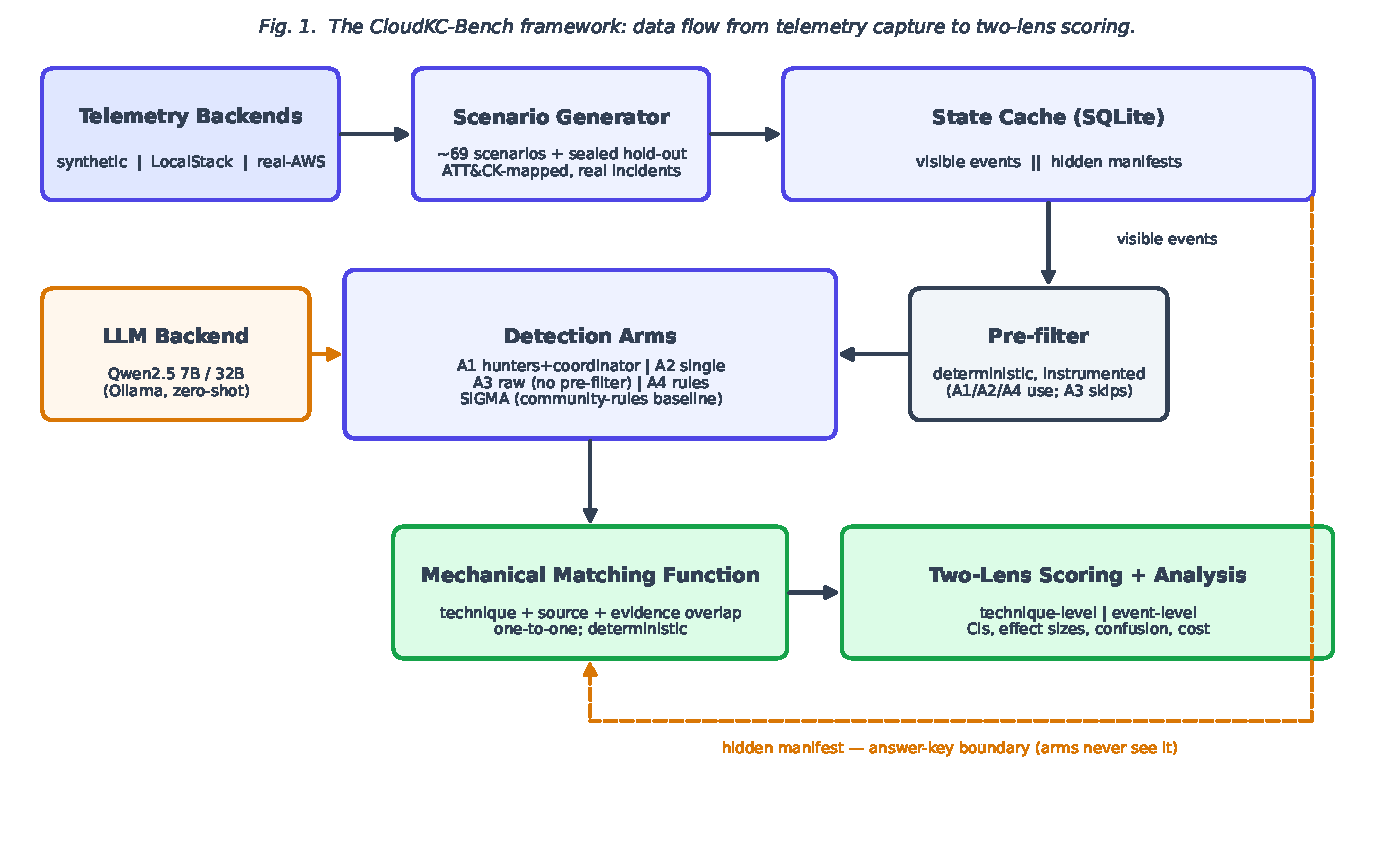
\includegraphics[width=0.9\textwidth]{system_architecture.pdf}
\caption{The CloudKC-Bench framework: data flow from telemetry capture to two-lens scoring. The hidden
manifest reaches only the scorer, never the arms (the answer-key boundary).}
\label{fig:system}
\end{figure*}

\subsection{Scenario Generator and Dual Backends}
The generator produces roughly seventy scenarios across five never-mixed categories---single-domain,
multi-stage kill chains, low-and-slow evasion, ephemeral compute, and benign noise---plus a sealed
hold-out set. Each scenario is grounded in a documented real incident and mapped to ATT\&CK-for-Cloud
techniques. Two interchangeable backends emit the same event schema: a \emph{synthetic} backend that
builds events deterministically and forms the reproducibility layer, and an \emph{execution} backend
that runs each scenario as real API calls against a local emulator or a real AWS sandbox and captures
the resulting telemetry.

\subsection{Ground Truth and the Answer-Key Boundary}
Each scenario ships a machine-checkable \emph{manifest}: an ordered list of stages, each naming its
technique, telemetry source, evidence events, and time span, validated against a published schema. The
essential rule is the \emph{answer-key boundary}: the technique label exists only in the manifest and
a hidden flag, never in the event data an arm reads. An attacker's API call and a routine
administrative call look identical in the visible telemetry, so the only way to tell them apart is to
reason about behavior, exactly as a real analyst must.

\subsection{Pre-filter and Arms}
Before any expensive reasoning, an optional pre-filter keeps an event if its name is on a short list
of high-risk actions or if a lightweight signature marks it suspicious. The full system, \textbf{A1},
applies the pre-filter and distributes surviving events to four specialist hunters whose findings a
coordinator merges. \textbf{A2} keeps the pre-filter but uses one general agent; comparing A1 with A2
measures multi-agent decomposition. \textbf{A3} removes the pre-filter; comparing A2 with A3 measures
the pre-filter's cost. \textbf{A4} replaces the language model with fixed rules; comparing the model
arms with A4 measures the model's value. An independent community \textbf{Sigma} baseline guards
against a rigged rules arm.

\subsection{The Mechanical Matching Function}
Scoring is a fixed function of the reconstructed chain and the manifest. Let the ground truth be a set
of stages $M=\{s_1,\dots,s_n\}$ with $s_i=(t_i,\sigma_i,E_i)$, where $t_i$ is the technique
identifier, $\sigma_i$ the telemetry source, and $E_i$ the set of evidence event identifiers. Let the
arm's output be $R=\{r_1,\dots,r_m\}$ with $r_j=(\hat t_j,\hat\sigma_j,\hat E_j)$. A reported stage
$r_j$ \emph{matches} a ground-truth stage $s_i$ when
\begin{equation}
\mathrm{match}(r_j,s_i)\iff \tau(\hat t_j,t_i)\ \wedge\ (\hat\sigma_j=\sigma_i)\ \wedge\ (\hat E_j\cap E_i\neq\varnothing),
\end{equation}
where $\tau(\cdot,\cdot)$ is the technique-agreement test: in \emph{exact} mode it holds only when
$\hat t=t$, and in \emph{parent} mode also when the two share a parent technique. The evidence
overlap prevents ``right answer, wrong reason'' credit. Matching is one-to-one, computed as a maximum
matching over the bipartite graph of allowed pairs. With true positives
$\mathrm{TP}=|\mathrm{matched}|$, false positives $\mathrm{FP}=m-\mathrm{TP}$, and false negatives
$\mathrm{FN}=n-\mathrm{TP}$,
\begin{equation}
\mathrm{Recall}=\frac{\mathrm{TP}}{\mathrm{TP}+\mathrm{FN}},\quad
\mathrm{Precision}=\frac{\mathrm{TP}}{\mathrm{TP}+\mathrm{FP}},\quad
F_1=\frac{2PR}{P+R}.
\end{equation}
A benign scenario has $n=0$, so any reported stage is a false positive, which is how false alarms are
measured.

\subsection{The Two Scoring Lenses}
Because naming a technique and simply finding an attack are different skills, every result is reported
under two lenses. The \emph{technique-level} lens is the strict function above. The \emph{event-level}
lens is technique-blind: if $G$ is the set of ground-truth attack events and $P$ the set an arm
flagged, then
\begin{equation}
\mathrm{event\_recall}=\frac{|P\cap G|}{|G|},\qquad
\mathrm{event\_precision}=\frac{|P\cap G|}{|P|}.
\end{equation}
Reporting both separates \emph{finding} an attack from \emph{labeling} it.

% ====================================================================
\section{Implementation}\label{sec:impl}
CloudKC-Bench is implemented in Python and depends only on a small set of established libraries:
\texttt{jsonschema} validates manifests, \texttt{requests} carries model calls, \texttt{boto3} drives
the cloud backends, and the standard-library \texttt{sqlite3} stores events, scenarios, arm outputs,
and scores. The suite runs under \texttt{pytest} on Python 3.11--3.13 in continuous integration. The
synthetic backend needs no infrastructure; the LocalStack backend issues real API calls against a
local emulator; and the real-AWS backend runs identical code against a live sandbox, protected by
explicit safety gates and a mandatory teardown of every created resource.

The language-model arms use open Qwen2.5 models~\cite{qwen}, served locally through Ollama behind an
OpenAI-compatible interface, keeping the study free of external quotas and all telemetry private. Two
sizes are studied on identical data---7-billion and 32-billion parameters, both four-bit
quantized---with \emph{no} fine-tuning; the models are used zero-shot, given only the closed list of
in-scope techniques in the prompt so the task is well posed. Each experiment pins one model version
and records it with every result. The real-model experiments ran on a workstation with a 24\,GB
graphics card sufficient to hold the 32B model in graphics memory, and the real-cloud experiments used
a dedicated AWS sandbox account confined to one approved region with a pre-configured cost budget.

A complete run proceeds in two separated phases. The first executes scenarios against the chosen
backend and stores the telemetry with hidden manifests; this is the only phase that touches, and
bills, the cloud. The second lets each arm read the stored events, propose a chain, and be scored.
Both phases are resumable, so an interrupted run skips completed work. The experiments here use the
development set of fifty-nine scenarios, each run with three seeds. The entire framework is released as
an open artifact so that every number in this paper can be reproduced.

% ====================================================================
\section{Experimental Results}\label{sec:results}

\subsection{Metrics and Setup}
All results come from the fifty-nine development scenarios, run three times each against a real AWS
account with the two Qwen2.5 models on identical captured telemetry; the hold-out set is untouched.
We report metrics under two lenses: technique-level metrics use parent-technique credit unless stated,
while event-level metrics ignore the technique label and ask only whether the right events were found.
Beyond recall (the fraction of true attack events found) and precision (the fraction of flagged events
that are genuine), we report a fuller set of standard classification metrics recovered from the full
event-level confusion matrix, because event detection is highly \emph{imbalanced}---attack events are a
small minority---a regime in which raw accuracy is misleading. The \emph{$F_1$ score} is the harmonic
mean of recall and precision, rewarding a method only when both are high. The \emph{false-positive rate}
(FPR) is the fraction of benign events that are wrongly flagged, and \emph{specificity} is its
complement, the fraction of benign events correctly left alone; a noisy detector has high FPR and low
specificity. \emph{Balanced accuracy} averages the true-positive and true-negative rates so that the
majority (benign) class cannot dominate the score. The \emph{Matthews Correlation Coefficient} (MCC)
combines all four confusion-matrix cells into a single value between $-1$ and $+1$, where $0$ is chance
and $1$ is perfect, and is widely regarded as the most reliable single summary for imbalanced binary
detection. For the two pre-registered hypotheses we report bootstrap 95\% confidence intervals, Cohen's
$d_z$, and Holm--Bonferroni-corrected permutation $p$-values; other comparisons are descriptive.

\subsection{The Two Scoring Lenses: the Central Finding}
The two lenses tell almost opposite stories, as Table~\ref{tab:twolens} and Fig.~\ref{fig:twolens}
show. Under the strict technique-level lens the language-model arms score very low on multi-stage
kill chains---recall of 0.070, 0.035, and 0.080 for A1, A2, and A3---while the rule-based arm A4
reaches 0.867. The event-level lens overturns this reading: the same model arms find between 0.762 and
0.894 of the true attack events, at very high precision (0.815, 0.952, and a perfect 1.000 for A3),
whereas the rules reach high event recall (0.967) but far lower event precision (0.649). When the
model flags an event it is almost always right, more reliably than the rules, yet it usually attaches
the wrong technique. The bottleneck is technique attribution, not cross-domain event detection.

\begin{table}[t]
\caption{Multi-stage kill chains, two scoring lenses (Qwen2.5-32B, real-AWS, $n{=}15$, 3 seeds).}
\label{tab:twolens}
\centering
\begin{tabular}{lccccc}
\toprule
Arm & Tech.\ rec. & Tech.\ prec. & Ev.\ rec. & Ev.\ prec. & Tokens \\
\midrule
A1 & 0.070 & 0.066 & 0.894 & 0.815 & 1814 \\
A2 & 0.035 & 0.039 & 0.762 & 0.952 & 1314 \\
A3 & 0.080 & 0.113 & 0.816 & \textbf{1.000} & 1393 \\
A4 (rules) & \textbf{0.867} & 0.474 & 0.967 & 0.649 & 0 \\
SIGMA & 0.739 & 0.433 & --- & --- & 0 \\
\bottomrule
\end{tabular}
\end{table}

\begin{figure}[t]
\centering
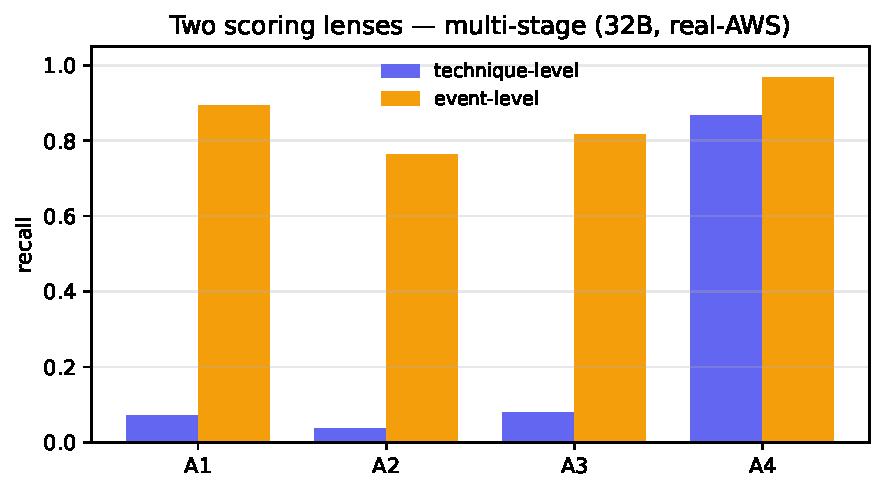
\includegraphics[width=\linewidth]{two_lens.pdf}
\caption{Technique-level vs.\ event-level recall per arm on multi-stage kill chains (32B, real-AWS).}
\label{fig:twolens}
\end{figure}

This precision advantage is seen most clearly when the arms are placed as operating points in ROC space
(Fig.~\ref{fig:roc}): the language-model arms sit high and to the left, near the ideal corner, while the
rule-based arm sits far to the right at a high false-positive rate. For a security operations center,
where analyst time is scarce, the model's high precision is the more valuable property.

The richer classification metrics defined above, reported in Table~\ref{tab:extended}, sharpen this
finding rather than soften it. On the MCC---the single balanced score for imbalanced detection---the raw
language-model arm reaches $0.745$ against the rules' $0.393$, nearly double, and it records an FPR of
$0.000$ against the rules' $0.750$: the rules flag three of every four non-attack events, whereas the
model flags essentially none. Balanced accuracy ($0.889$ vs $0.620$) and specificity ($1.000$ vs
$0.250$) tell the same story. Figure~\ref{fig:radar} visualizes this as a multi-metric profile in which
the language-model arms trace large, well-rounded polygons while the rule-based arm is
spiky---strong on recall but collapsing on specificity, balanced accuracy, and MCC---and the heatmap in
Figure~\ref{fig:heat} summarizes every metric at once.

Two further metric families address reproducibility and efficiency. Because language models are
non-deterministic, we quantify run-to-run stability as the standard deviation of technique-level recall
across the three seeds; it is small, between $0.03$ and $0.05$ for the model arms (and zero for the
deterministic rules), and Figure~\ref{fig:stabox} shows the per-run distributions are tight, turning the
usual hand-wave about model variability into a measured, and reassuringly small, quantity. Latency is
reported as percentiles rather than a mean: the multi-agent arm has a median of about $13.2$ seconds and
a 95th-percentile of $17.0$ seconds per scenario, roughly double the single-agent arm
(Figure~\ref{fig:latbox}), while event recall per thousand tokens is highest for the single-agent arm at
$0.58$, the most economical language-model configuration.

\begin{table}[t]
\caption{Extended event-level metrics beyond the recall and precision of Table~\ref{tab:twolens}
(Qwen2.5-32B, multi-stage), computed from the event-level confusion matrix, micro-averaged over events.
FPR: lower is better; all others: higher is better.}
\label{tab:extended}
\centering
\small
\begin{tabular}{lccccc}
\toprule
Arm & $F_1$ & FPR & Spec. & Bal.Acc. & MCC \\
\midrule
A1 & 0.913 & 0.211 & 0.789 & 0.864 & 0.746 \\
A2 & 0.849 & 0.044 & 0.956 & 0.856 & 0.682 \\
A3 & 0.875 & \textbf{0.000} & \textbf{1.000} & \textbf{0.889} & \textbf{0.745} \\
A4 (rules) & 0.823 & 0.750 & 0.250 & 0.620 & 0.393 \\
\bottomrule
\end{tabular}
\end{table}

\begin{figure}[t]
\centering
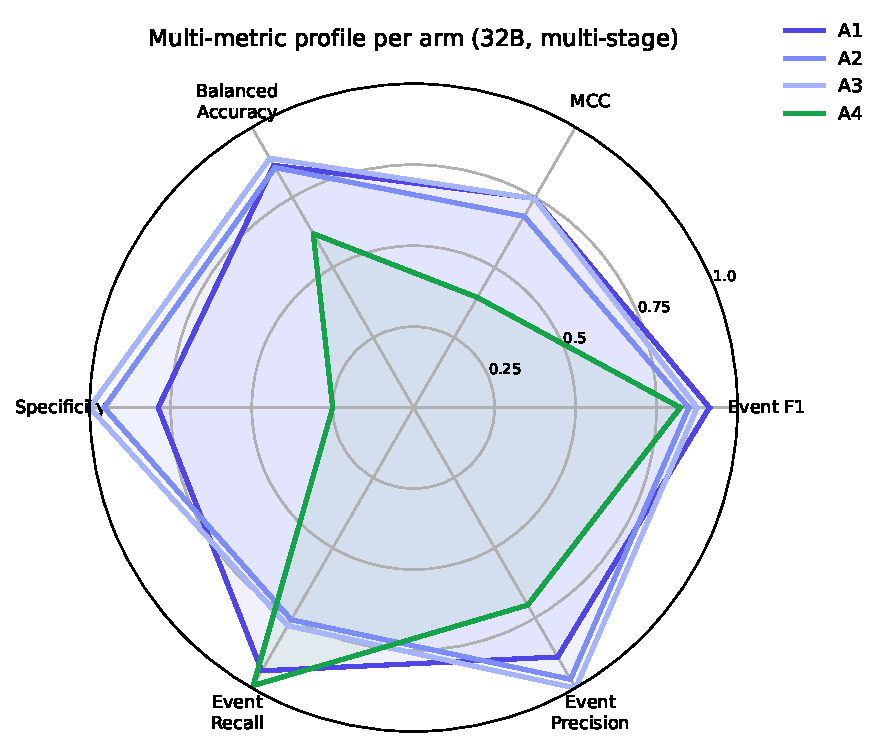
\includegraphics[width=0.86\linewidth]{fig_metrics_radar.pdf}
\caption{Multi-metric profile per arm (32B, multi-stage). The LLM arms are well-rounded; the rules
(A4) are strong on recall but weak on specificity, balanced accuracy, and MCC.}
\label{fig:radar}
\end{figure}

\begin{figure}[t]
\centering
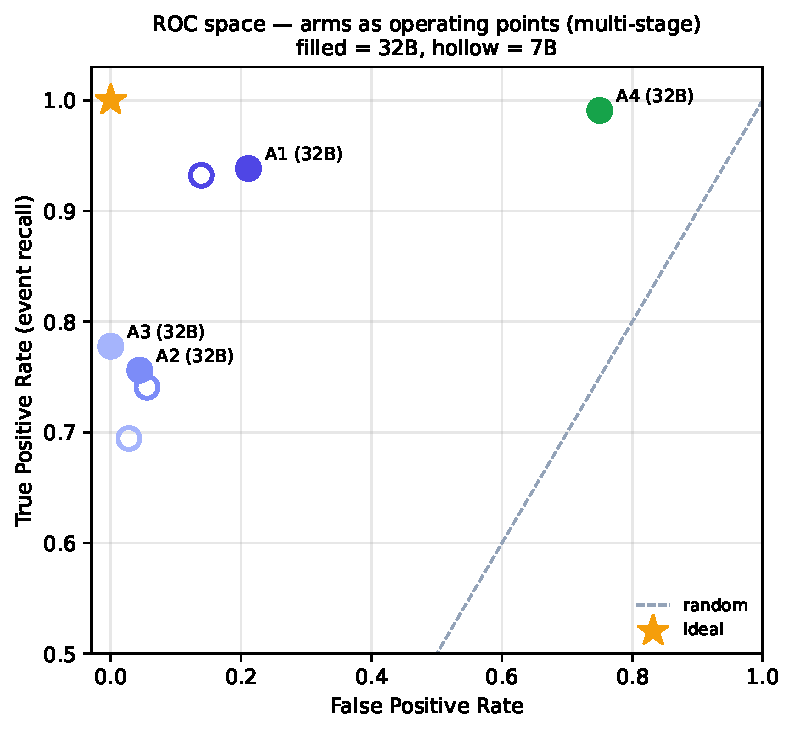
\includegraphics[width=0.9\linewidth]{fig_roc_space.pdf}
\caption{Each arm as an operating point in ROC space (multi-stage); filled markers are 32B, hollow are
7B. The LLM arms sit near the ideal corner; the rules sit far right at FPR $0.75$.}
\label{fig:roc}
\end{figure}

\begin{figure}[t]
\centering
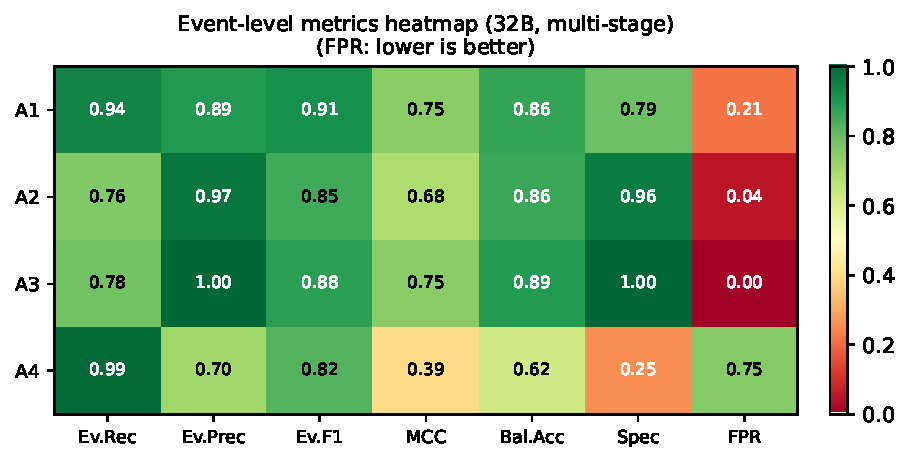
\includegraphics[width=\linewidth]{fig_metrics_heatmap.pdf}
\caption{Event-level metrics heatmap (32B, multi-stage). Green is better; for FPR, lower (redder) is
better.}
\label{fig:heat}
\end{figure}

\begin{figure}[t]
\centering
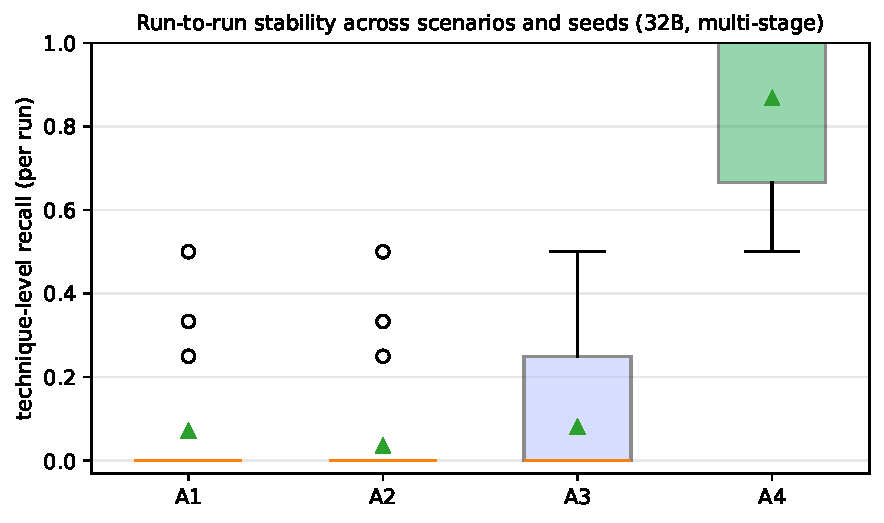
\includegraphics[width=\linewidth]{fig_seed_stability_box.pdf}
\caption{Run-to-run stability: distribution of technique-level recall across scenarios and seeds
(32B, multi-stage). Tight boxes indicate low non-determinism.}
\label{fig:stabox}
\end{figure}

\begin{figure}[t]
\centering
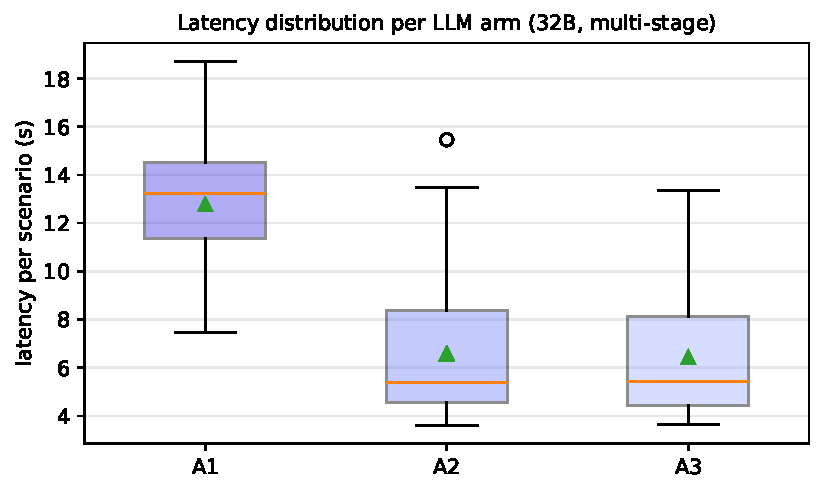
\includegraphics[width=0.92\linewidth]{fig_latency_box.pdf}
\caption{Per-scenario latency distribution for the LLM arms (32B, multi-stage). The multi-agent arm
(A1) is roughly twice as slow as the single-agent arms.}
\label{fig:latbox}
\end{figure}

\subsection{Per-Category Behavior}
Figs.~\ref{fig:reccat} and~\ref{fig:evcat} and Table~\ref{tab:percat} show the pattern is not peculiar
to multi-stage attacks. The rule-based arm dominates technique-level recall in every category, while
the model arms stay between roughly 0.10 and 0.17. At the event level, the model arms recover most
true attack events across every attack category (recall $\sim$0.76--0.99); the benign category is
empty by construction, and it is there that the rules' over-triggering is most visible.

\begin{figure*}[t]
\centering
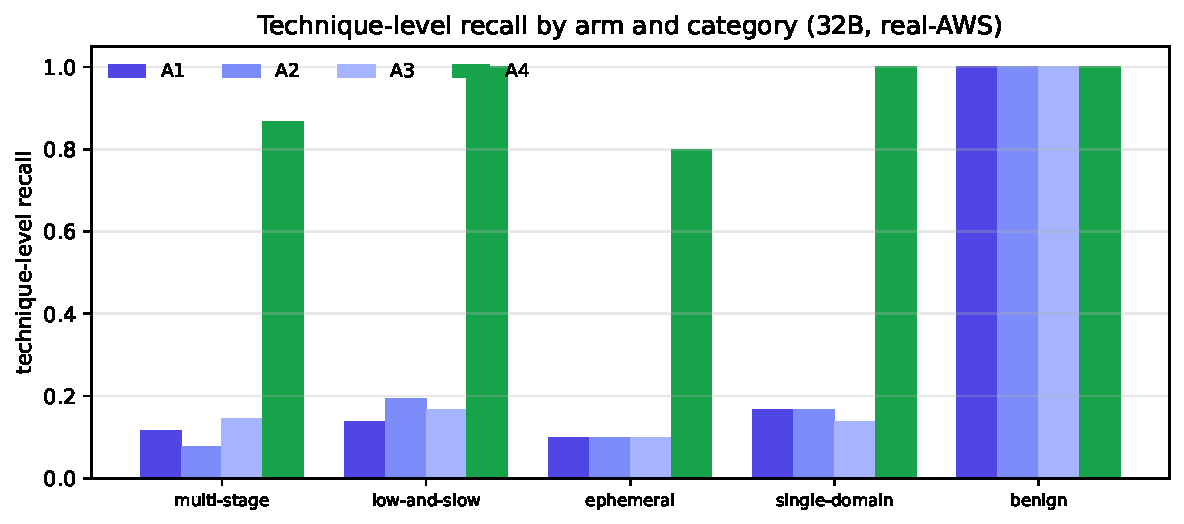
\includegraphics[width=0.82\textwidth]{recall_by_category.pdf}
\caption{Technique-level recall by arm across the five categories (32B, real-AWS).}
\label{fig:reccat}
\end{figure*}

\begin{figure*}[t]
\centering
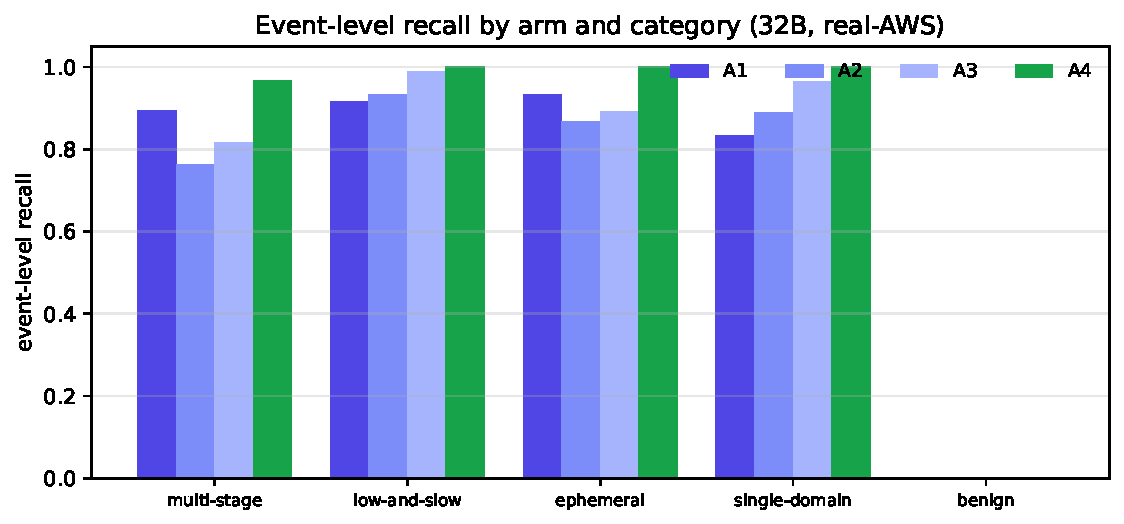
\includegraphics[width=0.82\textwidth]{percategory_event.pdf}
\caption{Event-level recall by arm across the five categories (32B, real-AWS).}
\label{fig:evcat}
\end{figure*}

\begin{table}[t]
\caption{Per-category recall (32B, real-AWS): technique-level with 95\% CI, and event-level.}
\label{tab:percat}
\centering
\small
\begin{tabular}{llccc}
\toprule
Arm & Category & Tech.\ rec.\ [95\% CI] & Ev.\ rec. & Ev.\ prec. \\
\midrule
A1 & multi-stage   & 0.117 [0.044,0.204] & 0.894 & 0.815 \\
A1 & low-and-slow  & 0.139 [0.000,0.333] & 0.917 & 0.448 \\
A1 & ephemeral     & 0.100 [0.000,0.300] & 0.933 & 0.404 \\
A1 & single-domain & 0.167 [0.000,0.417] & 0.833 & 0.501 \\
A4 & multi-stage   & 0.867 [0.778,0.950] & 0.967 & 0.649 \\
A4 & low-and-slow  & 1.000 [1.000,1.000] & 1.000 & 0.374 \\
A4 & ephemeral     & 0.800 [0.500,1.000] & 1.000 & 0.361 \\
A4 & single-domain & 1.000 [1.000,1.000] & 1.000 & 0.452 \\
\bottomrule
\end{tabular}
\end{table}

\subsection{The Two Primary Hypotheses}
Table~\ref{tab:hyp} states both pre-registered outcomes, and both resolve as negatives. The best
model arm trails the rules by a mean of $-0.750$ ($d_z=-3.91$, $p<0.001$, Holm-corrected), so H1 is
\emph{not supported}. The multi-agent arm differs from the single-agent arm by only $+0.027$ in F1
($p=0.59$), so we \emph{fail to reject} H2: multi-agent decomposition adds no measurable value.

\begin{table}[t]
\caption{Pre-registered hypothesis tests (multi-stage, 32B).}
\label{tab:hyp}
\centering
\small
\begin{tabular}{llcc}
\toprule
Test & Comparison & Mean diff [95\% CI] & Verdict \\
\midrule
H1 & A1 vs A4 recall & $-0.750$ [$-0.841,-0.654$] & Not supported \\
H2 & A1 vs A2 $F_1$  & $+0.027$ [$-0.051,0.118$]  & Fail to reject \\
\bottomrule
\end{tabular}
\end{table}

\subsection{Model Scale: 7B versus 32B}
Because both models ran over identical events, Table~\ref{tab:scale} and Figs.~\ref{fig:scalems}
and~\ref{fig:scalecat} isolate model size. A validity check appears first: the
rules produce identical scores under both models (0.867), as they must. On technique-level recall
(Fig.~\ref{fig:scalems}), scaling helps modestly---A1 rises 0.024 to 0.070 and A3 0.017 to
0.080---but stays an order of magnitude below the rules. The event level is more striking (Table~\ref{tab:scale};
the 7B and 32B operating points nearly coincide in the ROC space of Fig.~\ref{fig:roc}): the two models
are almost indistinguishable, with even the 7B model at $\sim$0.90 recall and $\sim$0.90 precision. The model's useful capability, locating attack events, does not
require a large model, whereas the capability that improves with scale, exact naming, remains too
weak to matter. Fig.~\ref{fig:scalecat} shows the modest gain is spread across categories.

\begin{table}[t]
\caption{Model scale on identical real-AWS telemetry (multi-stage).}
\label{tab:scale}
\centering
\small
\begin{tabular}{lcccc}
\toprule
 & \multicolumn{2}{c}{Technique recall} & \multicolumn{2}{c}{Event recall} \\
Arm & 7B & 32B & 7B & 32B \\
\midrule
A1 & 0.024 & 0.070 & 0.905 & 0.894 \\
A2 & 0.030 & 0.035 & 0.783 & 0.762 \\
A3 & 0.017 & 0.080 & 0.771 & 0.816 \\
A4 & 0.867 & 0.867 & 0.967 & 0.967 \\
\bottomrule
\end{tabular}
\end{table}

\begin{figure}[t]
\centering
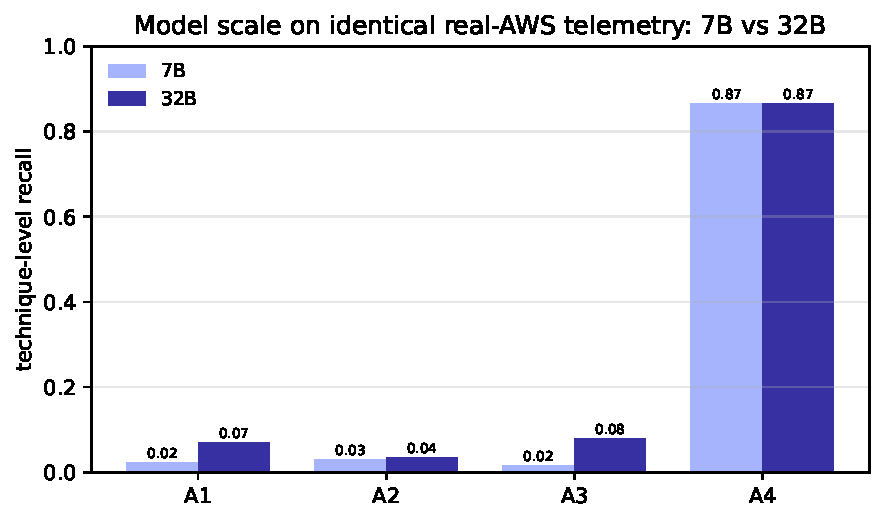
\includegraphics[width=\linewidth]{fig_model_scale_multistage.pdf}
\caption{Technique-level recall per arm, 7B vs.\ 32B on identical real-AWS telemetry.}
\label{fig:scalems}
\end{figure}


\begin{figure}[t]
\centering
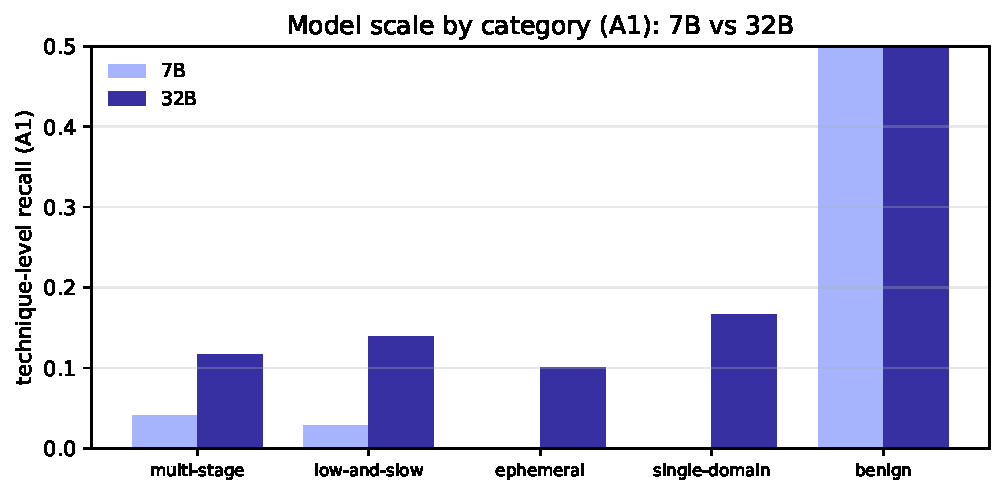
\includegraphics[width=\linewidth]{fig_model_scale_percategory.pdf}
\caption{Technique-level recall by category for arm A1, 7B vs.\ 32B.}
\label{fig:scalecat}
\end{figure}

\subsection{Where Attribution Breaks}
Fig.~\ref{fig:conf} dissects the reference arm's technique assignments. The failures are systematic
rather than random: the model names distinctive techniques reliably---brute-force credential attacks
every time---but struggles wherever several techniques share an observable footprint. Some errors are
within-family substitutions that parent-technique credit partly absorbs (for example, temporary elevated
access credited to its parent), while others cross ATT\&CK tactics entirely, such as labeling
network-discovery events as infrastructure modification. Fig.~\ref{fig:confscale} asks whether a larger
model repairs this, and the answer is largely no: scale wins on the distinctive techniques it already
handles but changes little on the many both models miss. The attribution bottleneck is structural,
rooted in the ambiguity of the telemetry, not dissolved by a bigger model.

We quantify these behaviors with four task-specific reliability metrics in Table~\ref{tab:taskspec}. No
multi-stage attack went entirely unnoticed---every arm achieves a $100\%$ \emph{detection-success rate},
flagging at least one true attack event in every scenario---yet the \emph{full-chain success rate},
reconstructing every stage correctly, is $0\%$ for the language model against $60\%$ for the rules. The
\emph{hallucination rate}, the fraction of proposals naming a technique outside the benchmark's closed
vocabulary despite the label set being supplied in the prompt, is low at 32B ($\le 1.8\%$) but rises
sharply for the smaller 7B model (to $6$--$10\%$): the vocabulary constraint suppresses hallucination
without eliminating it, and scale helps markedly. Finally, comparing \emph{tactic-level
accuracy}---whether the assigned technique at least shares the true technique's ATT\&CK tactic---against
exact technique accuracy tests for a family-level signal: the 32B model labels the exact technique on
only $4$--$8\%$ of attack events but a same-tactic technique on $14$--$22\%$. This weak doubling reveals
a limited family-level understanding; but because tactic accuracy still trails the rules' $97\%$ by a
wide margin, the model's difficulty is a broad attribution weakness, not merely within-tactic sibling
confusion.

\begin{table}[t]
\caption{Task-specific reliability metrics (Qwen2.5-32B, multi-stage). Hallucination = proposals naming
a technique outside the vocabulary; detection-success and full-chain are per-scenario rates;
technique-exact and tactic accuracy are per-event. The 7B model's hallucination rate is far higher
($6$--$10\%$).}
\label{tab:taskspec}
\centering
\small
\begin{tabular}{lccccc}
\toprule
 & Halluc. & Detect. & Full- & Tech. & Tactic \\
Arm & rate & success & chain & exact & acc. \\
\midrule
A1 & 1.8\% & 100\% & 0\% & 8.3\% & 14.2\% \\
A2 & 0.0\% & 100\% & 0\% & 4.0\% & 17.0\% \\
A3 & 0.4\% & 100\% & 0\% & 7.7\% & 21.9\% \\
A4 (rules) & 0.0\% & 100\% & \textbf{60\%} & \textbf{91.7\%} & \textbf{97.2\%} \\
\bottomrule
\end{tabular}
\end{table}

\begin{figure}[t]
\centering
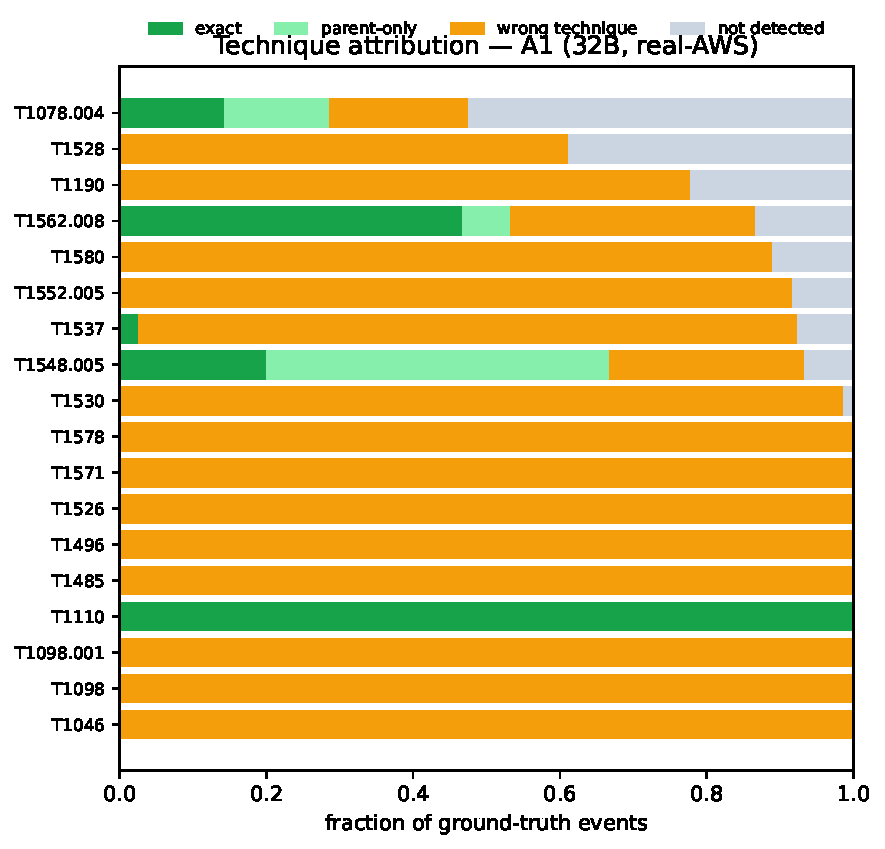
\includegraphics[width=\linewidth]{confusion_A1.pdf}
\caption{Technique attribution for arm A1 (32B): per technique, the fraction labeled exactly, with
parent credit, with the wrong technique, or missed.}
\label{fig:conf}
\end{figure}

\begin{figure}[t]
\centering
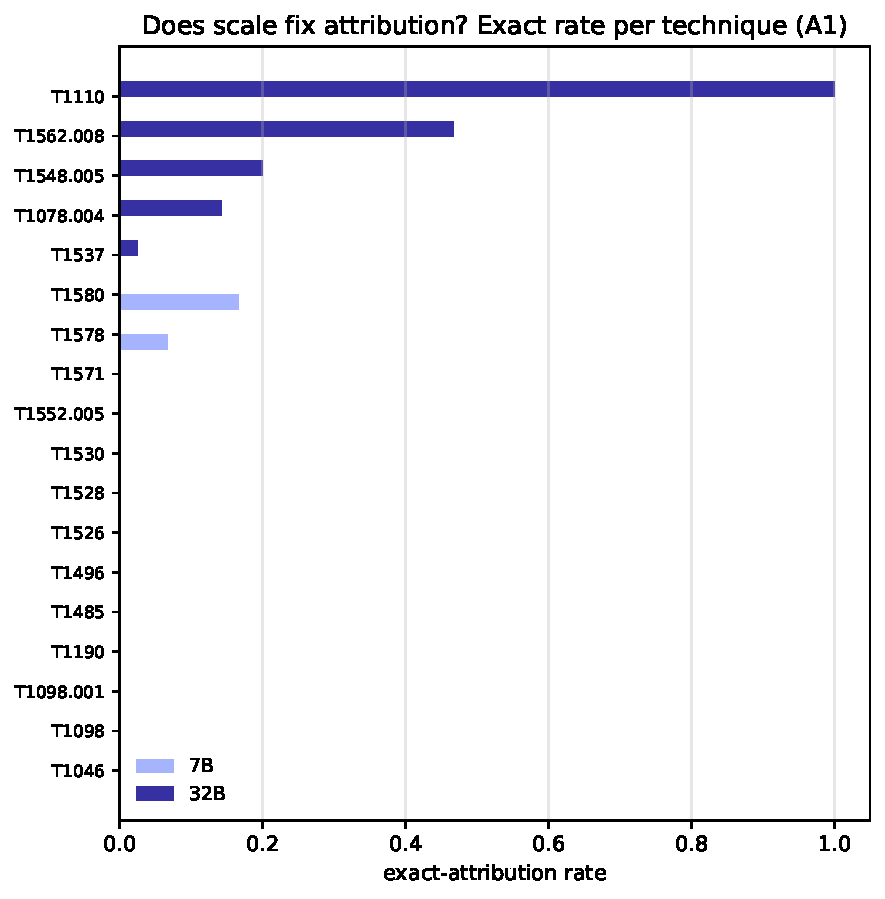
\includegraphics[width=\linewidth]{fig_confusion_scale_A1.pdf}
\caption{Exact-attribution rate per technique, 7B vs.\ 32B (arm A1). Scale does not fix the
technique confusions.}
\label{fig:confscale}
\end{figure}

\subsection{Cost, Latency, and the External Baseline}
Fig.~\ref{fig:cost} places each arm on a cost-versus-accuracy plane. The multi-agent arm is the most
expensive ($\sim$1814 tokens, 12.8\,s per scenario) because it queries the model once per telemetry
domain, whereas the single agent needs $\sim$1314 tokens; since the two are statistically
indistinguishable, the multi-agent premium buys nothing. Removing the pre-filter raises token cost
only slightly (1314 to 1393) but improves event recall (0.762 to 0.816), so the pre-filter discards
real detections for a small saving. The rules and Sigma incur no model cost. Finally, the independent
Sigma baseline reaches technique-level recall 0.739 on multi-stage---between the model arms at
$\sim$0.12 and the tuned rules at 0.867---confirming the rules' dominance is real and not an artifact
of a deliberately weak comparison.

\begin{figure}[t]
\centering
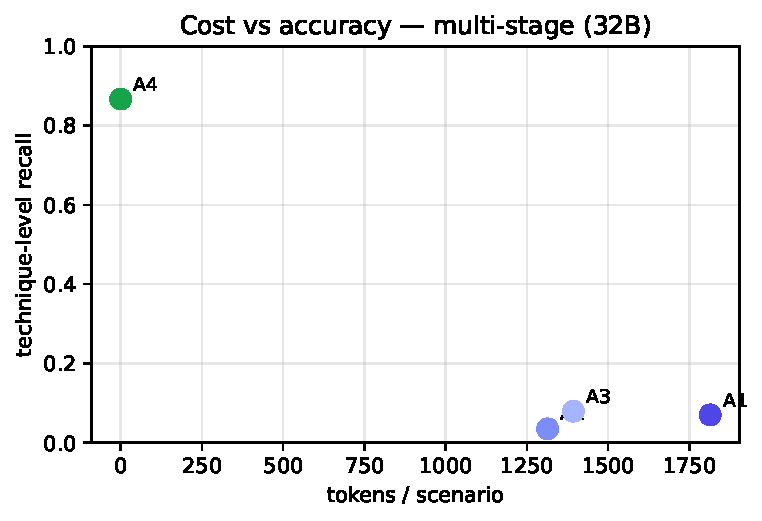
\includegraphics[width=\linewidth]{cost_accuracy.pdf}
\caption{Cost vs.\ technique-level recall per arm (multi-stage, 32B).}
\label{fig:cost}
\end{figure}

% ====================================================================
\section{Discussion}\label{sec:disc}
The headline of this study is a \emph{decomposition} rather than a winner. On real AWS multi-stage
kill chains, a mid-sized open language model performs cross-domain attack-event detection at higher
precision than deterministic rules, yet fails at exact technique attribution. The natural reading for
practice is that these capabilities belong to different tools: a model is well suited to
high-precision triage, while exact labeling is better left to rules or a human analyst. The model's
precision advantage has an intuitive cause---it reasons about an event in context and can decline to
flag a lone action a rule would trip on---which is also why removing the pre-filter improves its
recall.

The rules dominate the strict metric for a structural reason: their signatures are effectively the
inverse of the scenario generator, so they recover the exact sub-technique each scenario encodes, and
executing against real AWS did not dissolve this advantage because the captured telemetry is still the
structured API calls the benchmark issues. The strict metric therefore rewards any method that encodes
the answer key, which is why we lead with event-level detection; a decisive comparison would require
noisy production telemetry in which no static rule can invert the data. Practically, multi-agent
decomposition should not be adopted, the pre-filter is a tunable cost-versus-recall knob, and because
detection is scale-insensitive a deployment wanting only triage can use a small model.

These interpretations are subject to several threats to validity, which we examine systematically in
Section~\ref{sec:threats}.

% ====================================================================
\section{Threats to Validity}\label{sec:threats}
We organize the threats to our conclusions along the standard axes and describe how each is mitigated.

\emph{External validity} concerns whether our findings generalize beyond this study. The scenarios,
although grounded in documented real incidents and mapped to ATT\&CK techniques, are authored by the
research team, so their realism has a ceiling. We mitigate this with real-incident grounding, a sealed
hold-out set authored before the system is finalized and evaluated only once, and execution against a
real AWS account rather than a simulator alone. Even so, a single sandbox account and one model family
bound the generality of the scaling conclusion, which we present as indicative rather than definitive.

\emph{Construct validity} concerns whether the metrics measure what we intend. The rule-based arm's
near-optimal technique-level recall is partly an artifact of the benchmark, because its signatures
effectively invert the scenario generator; we address this by reporting two complementary lenses and
leading with event-level detection, and by including an independent community rule baseline that is not
tuned to our scenarios. The bespoke matching function is a further construct risk, mitigated by leading
with standard classification metrics (Section~\ref{sec:results}) and by publishing the function so that
it can be independently inspected.

\emph{Internal validity} concerns confounds within the experiment. The chief internal threat is
language-model non-determinism, which can render results irreproducible; we pin a single model version,
average over three seeds, and report the measured run-to-run variance, which is small. Holding model,
telemetry, and compute fixed across arms ensures that any score difference is attributable to the single
factor under test.

\emph{Statistical conclusion validity} concerns whether our inferences are sound given the sample. Per-
category sample sizes are small, so an a-priori power analysis restricts confirmatory claims to the two
pre-registered primary tests, corrected with the Holm--Bonferroni procedure, and treats all other
comparisons as descriptive, reported with effect sizes and bootstrap confidence intervals rather than
family-wise significance. These safeguards directly answer the evaluation pitfalls catalogued for
security machine learning~\cite{arp22}.

\emph{Baseline coverage} concerns the fairness of comparison. We enabled a managed cloud detector with a
multi-day baseline and collected its findings over the real-AWS run, but it produced no findings mapping
to any emulated technique. We interpret this as a construct limitation of the telemetry rather than of
the detector: our executed-API scenarios reproduce the control-plane shape of attacks but not the
network- and threat-intelligence-level signals such a detector consumes. We therefore report it as an
honest null and retain the community rule set as the scored external baseline; raising scenario realism
to emit those signals is future work.

\emph{Reproducibility} concerns whether the study can be repeated. Model drift and deprecation threaten
long-term reproducibility, mitigated by version pinning and the release of the full
artifact---generator, manifests, schema, matching function, and analysis scripts. Adversarial evasion of
the language model is explicitly out of scope for this study.

% ====================================================================
\section{Conclusion}\label{sec:conc}
We introduced CloudKC-Bench, the first open, ground-truthed benchmark for rebuilding AWS control-plane
multi-stage kill chains, and used it to run a pre-registered, controlled four-arm comparison, together
with an independent rule-based baseline, on real AWS telemetry. The work was motivated by a simple but
unanswered question: given heterogeneous cloud logs that share no common key, can a large language model
correlate across them to reconstruct an attack, and does it do so better than the simpler methods
already in use? By holding model, telemetry, and compute fixed and varying a single factor at a time,
the benchmark turns that question from a rhetorical one into a measurable one.

The central result is a decomposition rather than a winner. A mid-sized open language model detects
cross-domain attack events broadly and at higher precision than deterministic rules---on the
multi-stage category its false-positive rate is effectively zero against the rules' $0.75$, and its
Matthews correlation coefficient is nearly double---yet it fails at exact ATT\&CK-technique attribution,
where hand-tuned rules dominate because they encode the answer. These attribution errors are systematic
confusions among related techniques---often across ATT\&CK tactics, not only within them---rather than
random noise, and they persist as the model is scaled
from seven to thirty-two billion parameters: scaling improves naming only slightly and leaves event
detection, already strong at the smaller size, essentially unchanged. Both pre-registered hypotheses
resolved as negatives---the language model does not beat the rules on strict technique recall, and
multi-agent decomposition adds no measurable value over a single agent while costing more---and an
enabled managed detector produced no relevant findings, a null we report honestly rather than hide. For
a security operations center, the practical reading is clear: a language model is a promising
high-precision triage and correlation aid, surfacing the events that matter with few false alarms, while
exact technique labeling is better left to rules or human analysts.

Beyond any single verdict, the durable contribution of this work is the benchmark itself: an open,
mechanically scored artifact---generator, manifests, schema, matching function, and analysis
scripts---that converts previously unfalsifiable claims about language models in cloud security into
measurable ones, and that will remain useful as models improve. Two threads of future work follow
directly from our findings. The first is to close the signal gap that left both the rules near-optimal
and the managed detector silent, by injecting benign background traffic and raising scenario realism so
that the telemetry carries the network- and threat-intelligence-level signals a noisy production
environment would present; this is the decisive test of whether the model's precision advantage
survives outside a structured capture. The second is breadth: evaluating larger and more capable models,
incorporating passive network telemetry from a dedicated sensor, running the sealed hold-out set as a
final confirmatory check, and adding adversarial-evasion scenarios that probe robustness. We hope the
benchmark and its honest, mixed results encourage the community to measure, rather than assume, the
value of language models for reconstructing cloud attacks.

% ====================================================================
\begin{thebibliography}{99}
\bibitem{gartner25} Gartner, ``Gartner Forecasts Worldwide Public Cloud End-User Spending to Total \$723 Billion in 2025,'' press release, Nov.\ 2024.
\bibitem{gartner99} Gartner, ``Through 2025, 99\% of cloud security failures will be the customer's fault,'' cloud-security guidance. [Online; verify primary report].
\bibitem{capitalone} B. Krebs, ``What We Can Learn from the Capital One Hack,'' KrebsOnSecurity, 2019.
\bibitem{scarleteel} Sysdig Threat Research Team, ``SCARLETEEL: Operation Targeting AWS Fargate and Kubernetes,'' 2023.
\bibitem{teamtnt} Cado Security, ``TeamTNT Cryptojacking Worm Targeting AWS Credentials,'' 2020.
\bibitem{llmsurvey1} ``Exploring the Role of Large Language Models in Cybersecurity: A Systematic Survey,'' arXiv:2504.15622, 2025.
\bibitem{llmsurvey2} ``Large Language Models in Cybersecurity: A Survey of Applications, Vulnerabilities, and Defense Techniques,'' \emph{AI} (MDPI), vol.\ 6, no.\ 9, art.\ 216, 2025.
\bibitem{llmsurvey3} ``LLM-based Event Log Analysis Techniques: A Survey,'' arXiv:2502.00677, 2025.
\bibitem{llmcloudhunter} Y. Schwartz \emph{et al.}, ``LLMCloudHunter: Harnessing LLMs for Automated Extraction of Detection Rules from Cloud-Based CTI,'' in \emph{Proc.\ ACM Web Conf.\ (WWW)}, 2025.
\bibitem{huntgpt} T. Ali and P. Kostakos, ``HuntGPT: Integrating ML-Based Anomaly Detection and Explainable AI with LLMs,'' arXiv:2309.16021, 2023.
\bibitem{hutchins} E. M. Hutchins, M. J. Cloppert, and R. M. Amin, ``Intelligence-Driven Computer Network Defense Informed by Analysis of Adversary Campaigns and Intrusion Kill Chains,'' Lockheed Martin, 2011.
\bibitem{mitre} The MITRE Corporation, ``MITRE ATT\&CK for Cloud (IaaS) Matrix.'' [Online]. Available: attack.mitre.org
\bibitem{wilkens} F. Wilkens \emph{et al.}, ``Multi-Stage Attack Detection via Kill Chain State Machines,'' in \emph{Proc.\ 3rd Wksp.\ Cyber-Security Arms Race (CYSARM)}, ACM, 2021.
\bibitem{hetfusion} ``Attack Scenario Reconstruction via Fusing Heterogeneous Threat Intelligence,'' \emph{Computers \& Security}, Elsevier, 2023.
\bibitem{cybersoceval} Deason \emph{et al.}, ``CyberSOCEval: Benchmarking LLMs for Malware Analysis and Threat Intelligence Reasoning,'' arXiv:2509.20166, 2025.
\bibitem{excytin} Wu \emph{et al.}, ``ExCyTIn-Bench: Benchmarking LLM Agents on Cyber Threat Investigation,'' arXiv:2507.14201, 2025.
\bibitem{orgforge} ``OrgForge-IT: A Verifiable Synthetic Benchmark for LLM-Based Insider Threat Detection,'' arXiv:2603.22499, 2026.
\bibitem{acseeval} ``ACSE-Eval: Can LLMs Threat Model Real-World Cloud Infrastructure?,'' arXiv:2505.11565, 2025.
\bibitem{provsurvey} M. U. Rehman \emph{et al.}, ``Provenance-based Intrusion Detection Systems: A Survey,'' \emph{ACM Computing Surveys}, 2022.
\bibitem{tbdetector} ``TBDetector: Transformer-Based Detector for Advanced Persistent Threats with Provenance Graph,'' arXiv:2304.02838, 2023.
\bibitem{sigma} SigmaHQ, ``Sigma --- Generic Signature Format for SIEM Systems.'' [Online]. Available: github.com/SigmaHQ/sigma
\bibitem{mukherjee} A. Mukherjee and M. Kantarcioglu, ``Provenance-Based Agentic Threat Hunting with RAG and Chain-of-Thought,'' 2025.
\bibitem{stratus} Datadog, ``Stratus Red Team: Adversary Emulation for the Cloud.'' [Online]. Available: github.com/DataDog/stratus-red-team
\bibitem{cloudgoat} Rhino Security Labs, ``CloudGoat: Vulnerable-by-Design AWS Environment.'' [Online]. Available: github.com/RhinoSecurityLabs/cloudgoat
\bibitem{qwen} Qwen Team, ``Qwen2.5 Technical Report,'' 2024. [Verify arXiv ID].
\bibitem{arp22} D. Arp, E. Quiring, F. Pendlebury, A. Warnecke, F. Pierazzi, C. Wressnegger, L. Cavallaro, and K. Rieck, ``Dos and Don'ts of Machine Learning in Computer Security,'' in \emph{Proc.\ 31st USENIX Security Symp.}, 2022.
\bibitem{aisecevent22} ``A Survey on Artificial Intelligence Techniques for Security Event Correlation: Models, Challenges, and Opportunities,'' \emph{Artificial Intelligence Review} (Springer), 2022.
\bibitem{maac} ``MAAC: Novel Alert Correlation Method to Detect Multi-step Attack,'' arXiv:2011.07793, 2020.
\bibitem{graphweaver} ``GraphWeaver: Billion-Scale Cybersecurity Incident Correlation,'' arXiv:2406.01842, 2024.
\bibitem{secure_bench} ``SECURE: Benchmarking Large Language Models for Cybersecurity Advisory,'' arXiv:2405.20441, 2024.
\bibitem{llmbenchsurvey} ``A Survey on Large Language Model Benchmarks,'' arXiv:2508.15361, 2025.
\end{thebibliography}

\end{document}
